\documentclass{beamer}
\usepackage[utf8]{inputenc}
\usepackage{graphicx}
\usepackage{caption}

\usetheme{Hannover}

\beamertemplatenavigationsymbolsempty

\title{Introduction à l'utilisation de Linux}
\author{Nicolas Cubric\\Association Robotronik Phelma}
\date{}
\institute{Grenoble INP Phelma}
\logo{
\includegraphics[width=0.25\textwidth]{Images/logoclub.png}}

\setbeamerfont{page number in head/foot}{size=\large}
\setbeamertemplate{footline}[frame number]

\begin{document}

\maketitle

\begin{frame}{Sommaire}
	\tableofcontents
\end{frame}

\section{Introduction}
\begin{frame}{Introduction}
	\begin{itemize}
		\item Linux c'est quoi ?
		\item Linux ça se retrouve où ?
		\item Les distributions
	\end{itemize}
\end{frame}

\subsection{Linux c'est quoi ?}
\begin{frame}{Linux c'est quoi ?}
	\begin{center}
		
\includegraphics[width=0.5\textwidth]{Images/GNU_TUX.png}
		\captionof{figure}{Mascotte de GNU et de Linux}
	\end{center}
\end{frame}

\subsection{Linux ça se trouve où ?}
\begin{frame}{Linux ça se trouve où ?}
\end{frame}

\subsection{Les distributions}
\begin{frame}{Les distributions}
\end{frame}

\section{L'arborescence}
\begin{frame}{L'arborescence}
	\begin{center}
		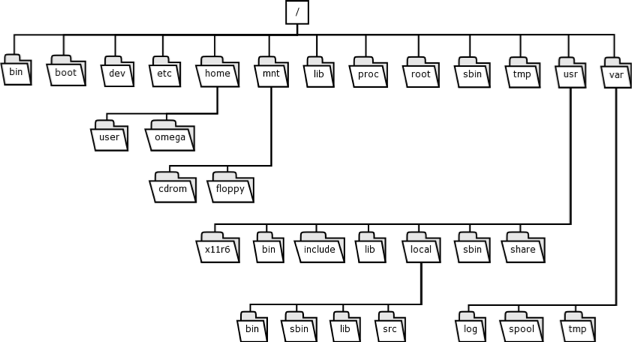
\includegraphics[width=0.7\textwidth]{Images/arborescence.png}
		\captionof{figure}{Arborescence}
	\end{center}
\end{frame}

\section{Les commandes de bases}
\begin{frame}{Les commandes de bases}
	\begin{itemize}
		\item pwd
		\item ls
		\item cd
		\item mkdir/rmdir
		\item touch/rm
	\end{itemize}
\end{frame}


\end{document}

